\documentclass{article}
\usepackage{listings}
\lstset{
    frame=single,
    breaklines=true
}
\usepackage{geometry}
\geometry{margin=1in}
\usepackage{graphicx}
\usepackage{float}
\lstset{language=Octave}
\title{ECG 772 HW 1}
\date{2015-09-19}
\author{Carlo Lopez-Tello}

\begin{document}
\maketitle
	\newpage
	\section{Histogram Equalization}
	
	\subsection{Write a function to perform histogram equalization on gray-scale images}
	\lstinputlisting[language=Octave]{Q1/histEqualize.m}
	
	\subsection{Perform histogram equalization on 'jetplane.tif'.}
	The images equalized with a smaller number of bins have less detail.
	\begin{figure}[H]
		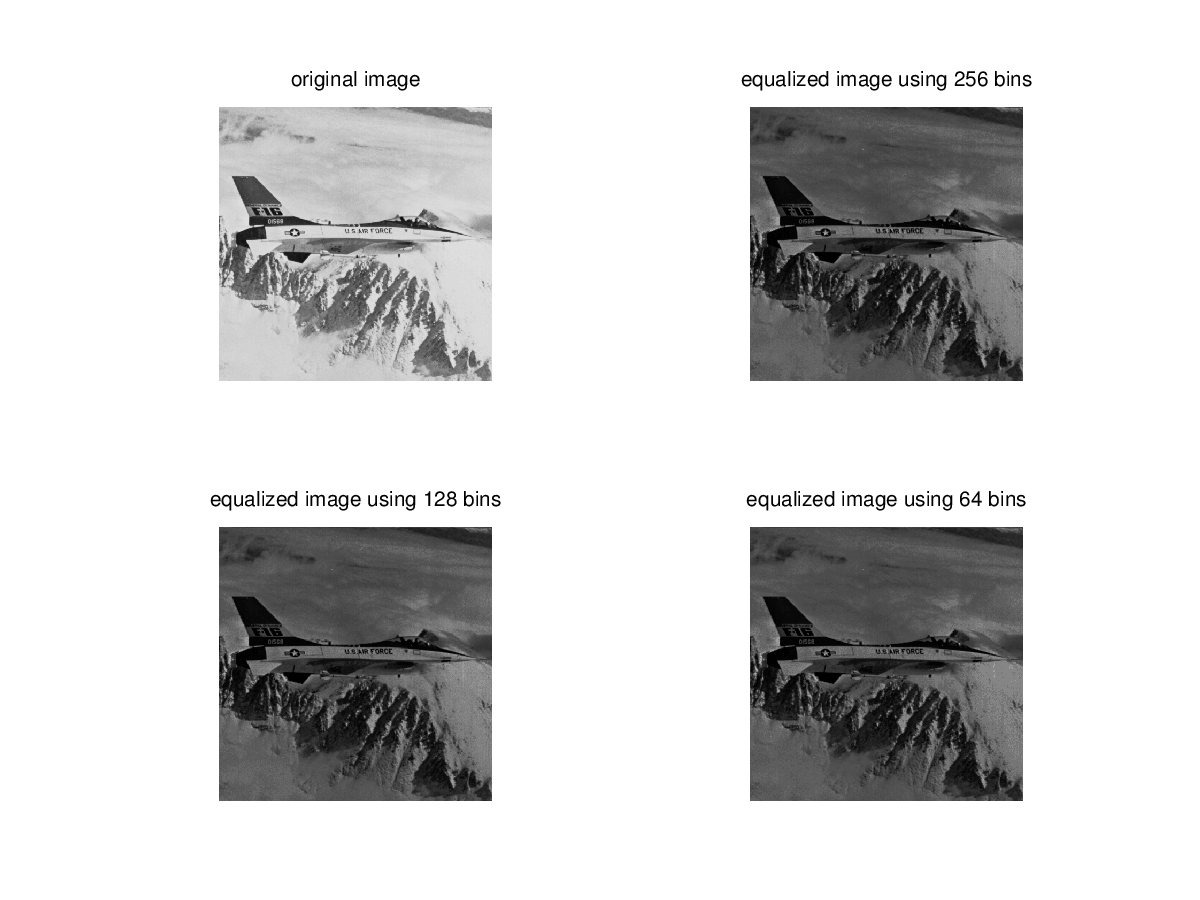
\includegraphics[width=\linewidth]{Q1/outputImages.png}
		\caption{equalized images}
	\end{figure}
	\begin{figure}[H]
		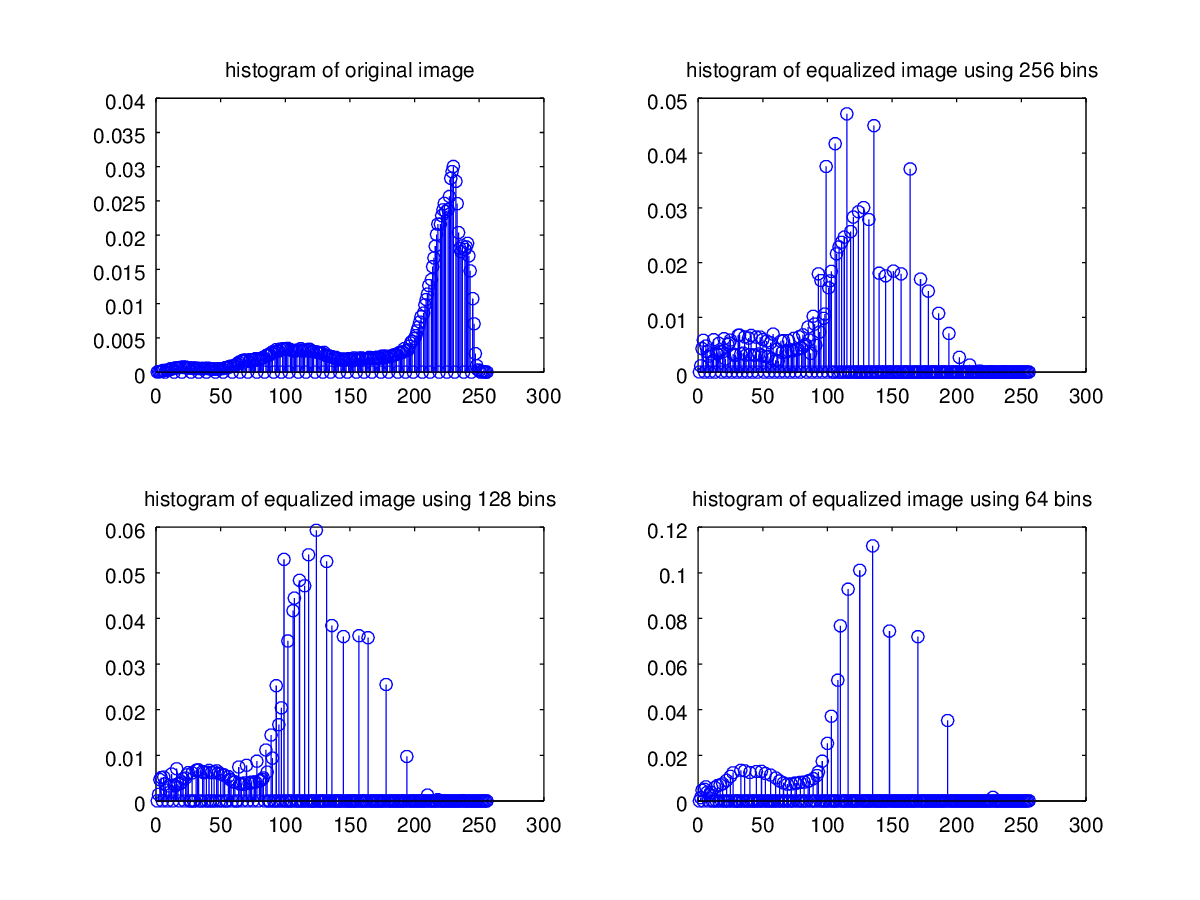
\includegraphics[width=\linewidth]{Q1/outputHistograms.png}
		\caption{histograms of equalized images}
	\end{figure}
	
	\subsection{Perform histogram equalization on 'jetplane.tif' using 32x32 blocks.}
	\begin{figure}[H]
		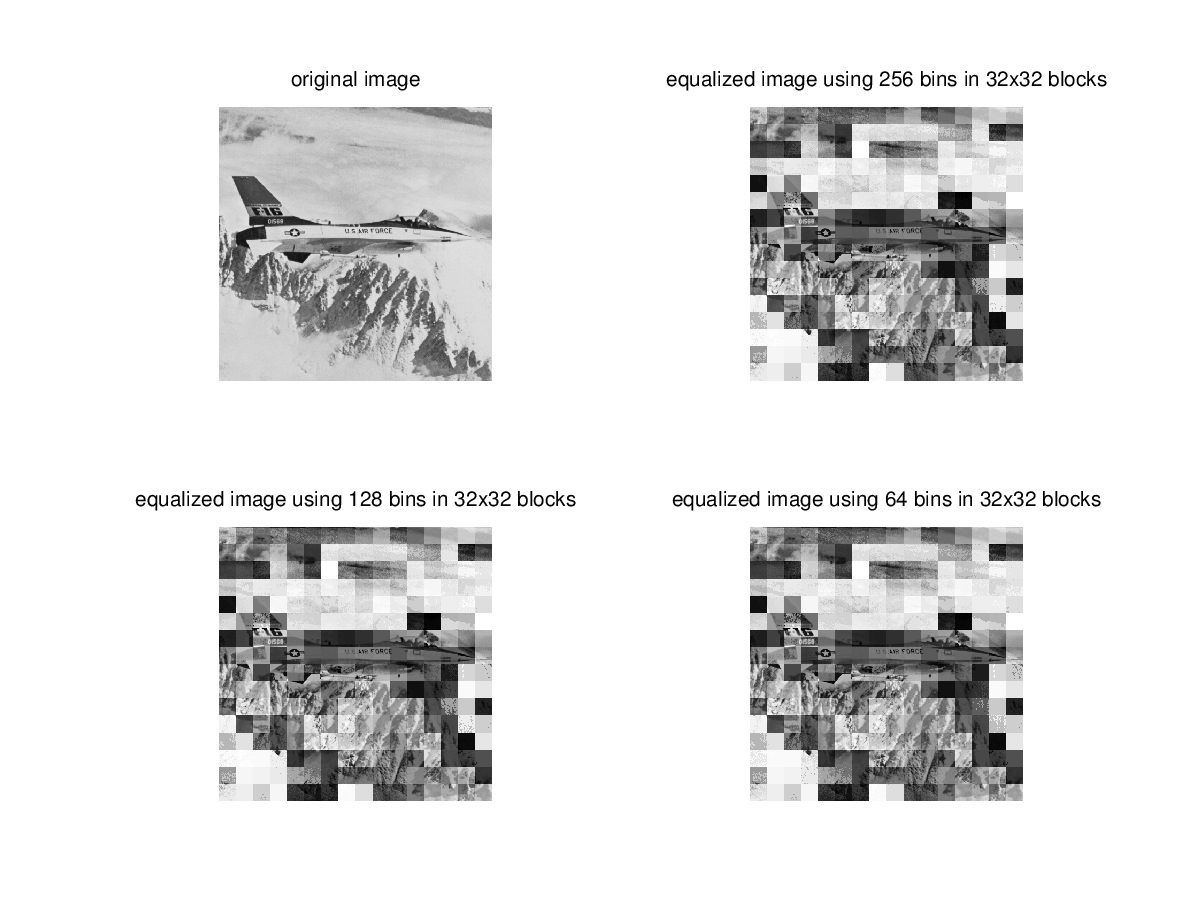
\includegraphics[width=\linewidth]{Q1/outputImages32.png}
		\caption{equalized images using 32x32 blocks}
	\end{figure}
	
	\newpage
	\section{Basic Morphology}
	
	\subsection{Detect faces of soccer players in team photos.}
	
	
	In order to detect the faces of soccer players I applied thresholding in HSV color space. To find the threshold ranges, I opened the image in GIMP and looked at the color of the pixels on the players foreheads. This gave me a threshold of S greater than 20, V greater 45, and H between 40 and 25. However, later I adjusted these values to S greater than 20, V greater than 20, and H between 35 and 5 to produce better results. After thresholding, I applied various morphological operations to get rid of traces of the crowd and to enhance objects with an aspect ratio of 3:2. The reason for this aspect ratio is that the faces of the players tend to be longer vertically and their knees tend to be longer horizontally. To achieve this I performed dilation using structural elements with a 3:2 aspect ratio and dilation with structural elements that were square.
	
	
	\begin{figure}[H]
		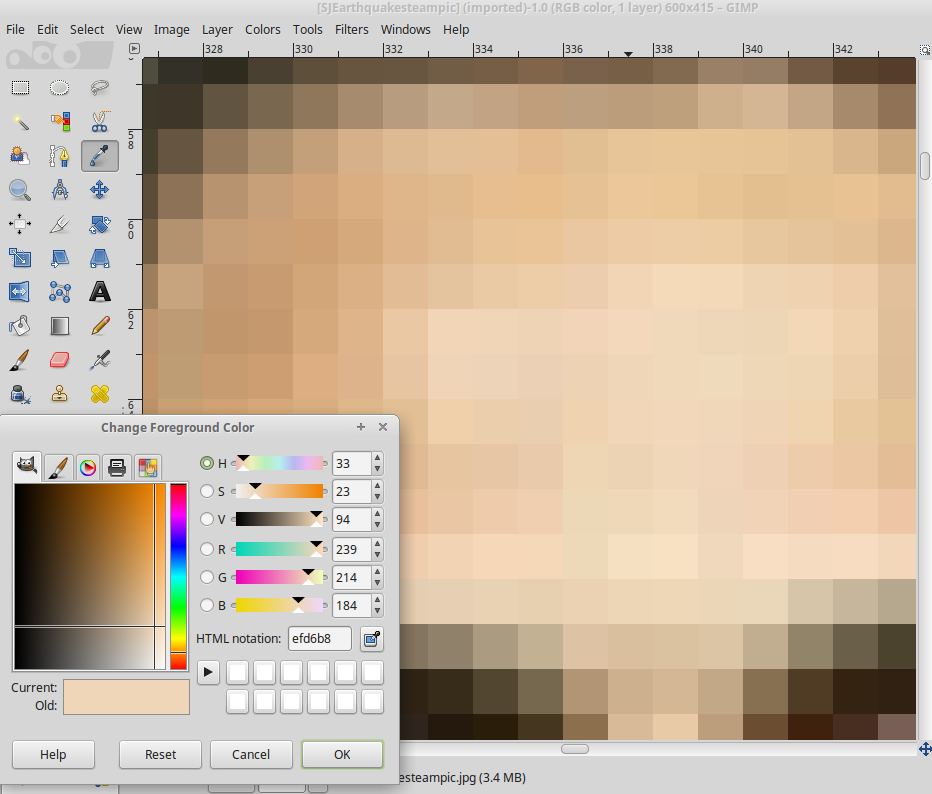
\includegraphics[width=\linewidth]{Q2/ForeheadHSV.png}
		\caption{selection of threshold}
	\end{figure}
	\begin{figure}[H]
		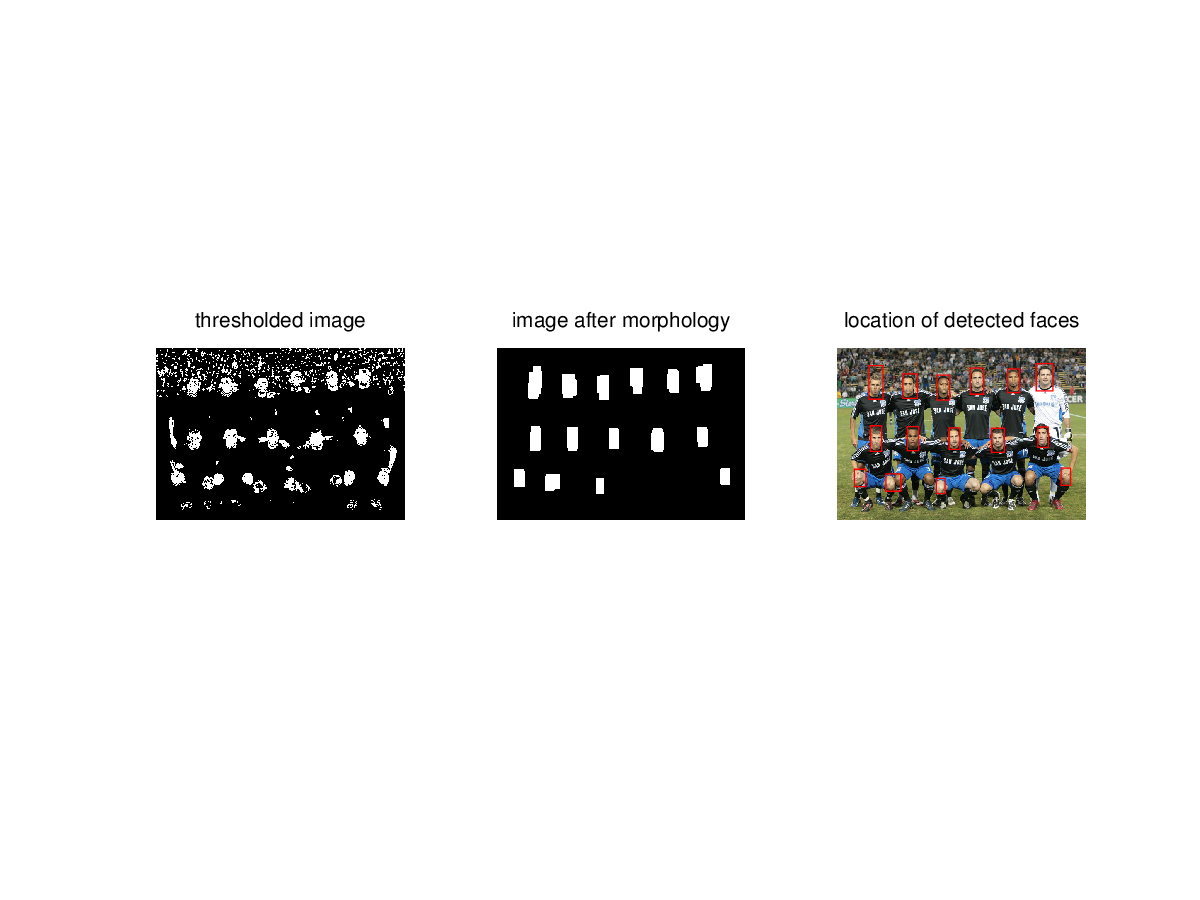
\includegraphics[width=\linewidth]{Q2/faceDetectSJEarthquakesteampic.png}
		\caption{face detection on 'SJEarthquakesteampic.jpg'}
	\end{figure}
	\begin{figure}[H]
		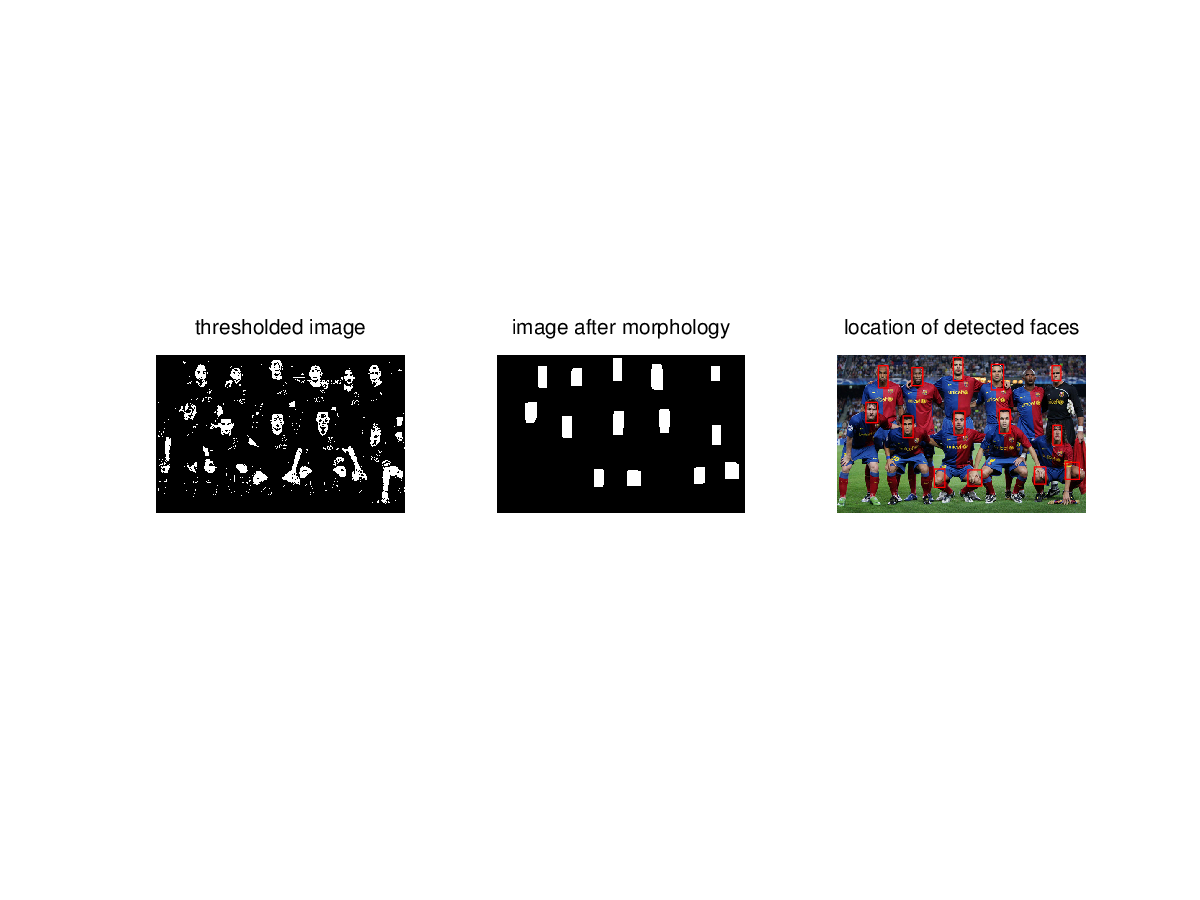
\includegraphics[width=\linewidth]{Q2/faceDetectbarcelona-team.png}
		\caption{face detection on 'barcelona-team.jpg'}
	\end{figure}
	
	
	The results for the two images are similar. In the image of the Earthquakes almost all of the player's faces are detected with a few knees selected as faces. The player whose face is not detected has a darker skin tone and a round face. Both of these characteristics could be the reason for his face not being correctly detected. In both images knees that appear longer in the y direction were detected as faces.
	
	\newpage
	\section{Filtering}
	\subsection{Use various filters to remove Gaussian noise with .005 variance from 'DSCN0479-001.JPG'.}
		
	
	Looking at the output images there seems to be a trade off between noise reduction and sharpness. The bigger filters make noise less noticeable, while at the same time making the image blurrier. The smaller filters remove less noise, but keep more of the sharpness of the image. The median filters appear to remove the same amount of noise as the mean filters, while preserving more sharpness.
		
	
	\begin{figure}[H]
		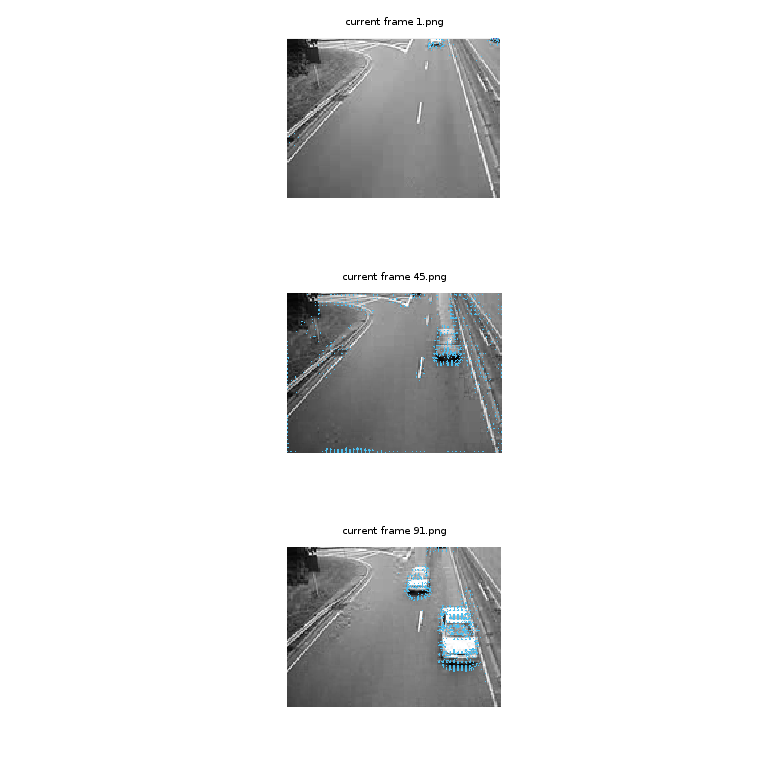
\includegraphics[width=\linewidth]{Q3/partA.png}
		\caption{images after filtering}
	\end{figure}
	
	\begin{table}[H]
		\centering
		\begin{tabular}{ c | c | c }
			filter & MSE & PSNR \\
			none & 72.0 & 29.6 \\
			3x3 mean filter & 32.9 & 33.0 \\
			5x5 mean filter & 36.7 & 32.5 \\
			3x3 median filter & 37.2 & 32.4 \\
			5x5 median filter & 36.2 & 32.5 \\
		\end{tabular}
		\caption{SNR and PSNR after filtering the noisy image}
	\end{table}
	
	The image with the smallest MSE and highest PSNR is the one produces by the 3x3 mean filter.
		
	\subsection{Use various filters to remove salt and pepper noise with .05 density from 'DSCN0479-001.JPG'.}
	
	
	Similar to the previous results, the bigger filters make the image blurrier and remove more noise. The median filters perform much better than the mean filters on salt and pepper noise. The best looking image is the one produced by the 3x3 median filter, since most of the noise is gone and the image is sharper than the one produced by the 5x5 median filter. 
	
	
	\begin{figure}[H]
		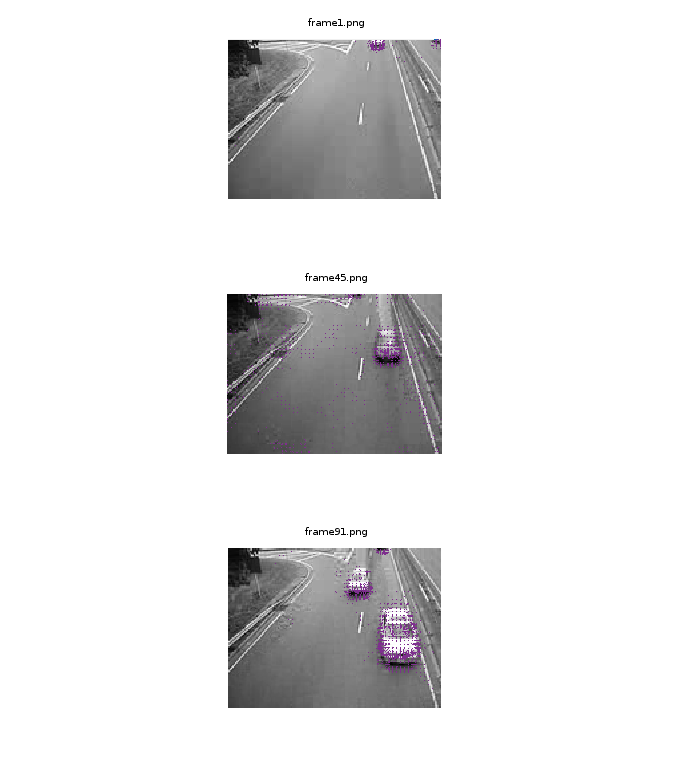
\includegraphics[width=\linewidth]{Q3/partB.png}
		\caption{images after filtering}
	\end{figure}
	
	\begin{table}[H]
		\centering
		\begin{tabular}{ c | c | c }
			filter & MSE & PSNR \\
			none & 6.5 & 40.0 \\
			3x3 mean filter & 42.4 & 31.9 \\
			5x5 mean filter & 44.9 & 31.6 \\
			3x3 median filter & 10.7 & 37.8 \\
			5x5 median filter & 24.7 & 34.2 \\
		\end{tabular}
		\caption{SNR and PSNR after filtering the noisy image}
	\end{table}
	
	
	The image with the smallest MSE and highest PSNR is the unfiltered noisy image. The cause of this is probably the density of errors in the filtered images. In other words the filtered images have small errors in every pixel, while the unfiltered image has large errors in a small number of images. This brings into question the reliability of MSE and PSNR as useful measures to compare the results of filtered images.
	
	
	\subsection{Use various filters to clean 'DSCN0482-001.JPG' a noisy version of 'DSCN0479-001.JPG'.}
	
	
	Just like before, the bigger filters produced blurrier images with less noise. However, the difference much smaller. The mean and median filters seem to produce very similar results. This makes the trade-off in performance undesirable. The 3x3 median filter takes 8 times longer than the 3x3 mean filter to produce an image, while the 5x5 median filter takes 16 times longer than the 5x5 mean filter to produce an image.
	
	
	\begin{figure}[H]
		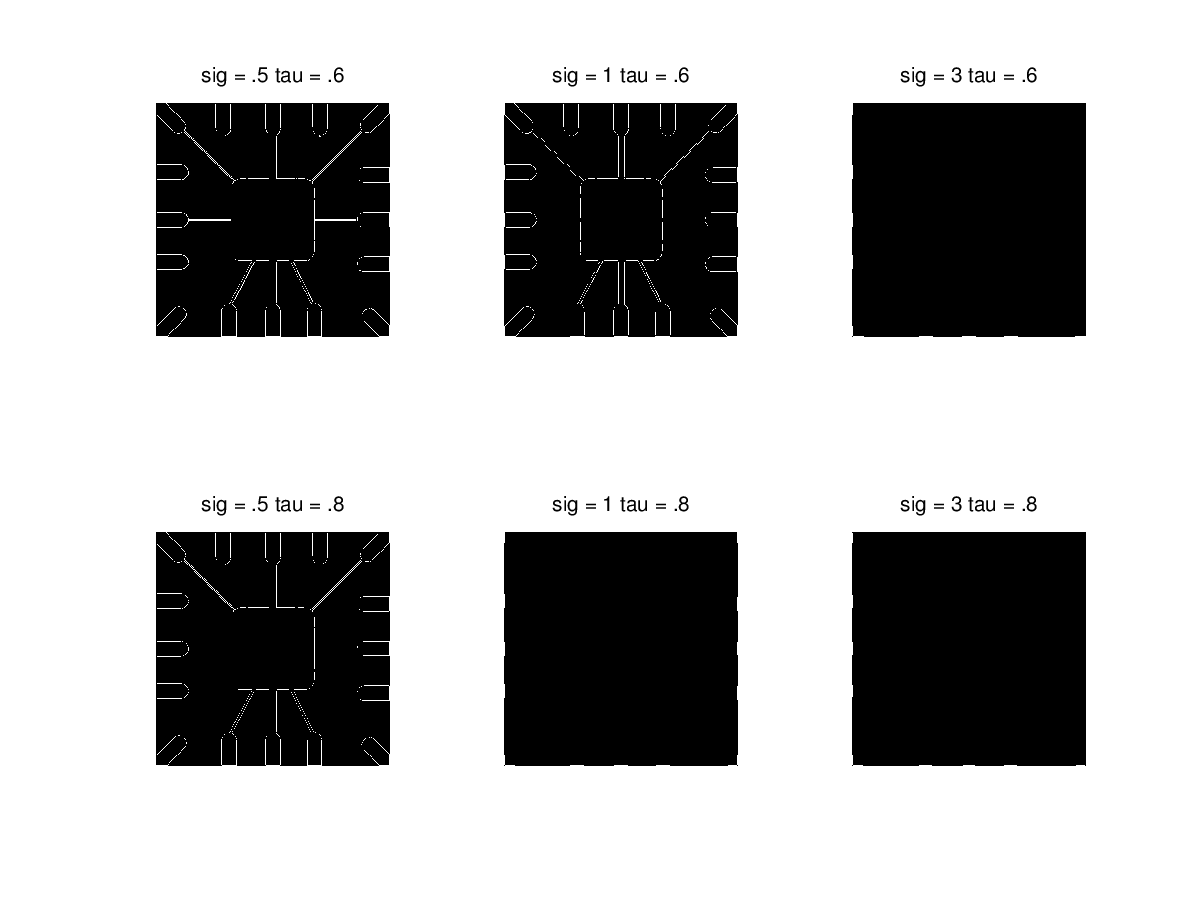
\includegraphics[width=\linewidth]{Q3/partC.png}
		\caption{images after filtering}
	\end{figure}
	
	\newpage
	\section{Code}
	\subsection{Q1 code}
	histEqualize.m
	\lstinputlisting[language=Octave]{Q1/histEqualize.m}
	
	Q1PartB.m
	\lstinputlisting[language=Octave]{Q1/Q1PartB.m}
	
	Q1PartC.m
	\lstinputlisting[language=Octave]{Q1/Q1PartC.m}
	
	\newpage
	\subsection{Q2 code}
	thresholdFaces.m
	\lstinputlisting[language=Octave]{Q2/thresholdFaces.m}
	
	faceDetect.m
	\lstinputlisting[language=Octave]{Q2/faceDetect.m}
	
	\newpage
	\subsection{Q3 code}
	Q3.m
	\lstinputlisting[language=Octave]{Q3/Q3.m}
	
	PartA.m
	\lstinputlisting[language=Octave]{Q3/PartA.m}
	
	PartB.m
	\lstinputlisting[language=Octave]{Q3/PartB.m}
	
	PartC.m
	\lstinputlisting[language=Octave]{Q3/PartC.m}
	
	\newpage
	\subsection{latex}
	\lstinputlisting{hw1.tex}
\end{document}
